% chap2.tex

\chapter{Background Material}\label{chap:figtab}

\section{Financial Portfolio}

A portfolio is a grouping of financial assets such as stocks, bonds, commodities, currencies and cash equivalents, as well as their fund counterparts, including mutual, exchange-traded and closed funds. Portfolios are held directly by investors or managed by financial professionals. These investor manage the distributions of funds into the various financial assets of the portfolio~\cite{stoyanov2007optimal}. 

Portfolio management can be either active or passive. In active management a team of managers or a single manager actively manage the funds of a portfolio. The portfolio managers rely on analytical research, forecast of market and their own knowledge of the behaviour of the market to make investment decision. Whereas passive portfolio management refers to a strategy where investors stress on minimizing the investor fee and avoid unpleasant results of failing to correctly predict the future. Passive portfolio management involves imitating the performance of a particular market index.

Portfolio managers use a lot of terminologies in the process of managing a portfolio and we therefore provide a background on the terminologies that we will use

\begin{itemize}
	\item \textbf{Asset allocation:} The practice of optimizing the risk/return profile of an investor by investing in a mix of asset that have low correlation to each other~\cite{reilly2011investment}. It is based on the understating that the different types of assets do not move in concert, and some of the assets are more volatile than other. 
	
	\item \textbf{Diversification:} It is the  practice of spreading funds among different asset classes. The practice of diversification provides a broad exposure to all the asset classes and thus spreads the risk and reward across asset classes~\cite{reilly2011investment}. It is difficult to know which particular subset of an asset class or sector is likely to outperform another, diversification seeks to capture the returns of all of the sectors over time but with less volatility at any one time.
	
	\item\textbf{Rebalancing:} It is the practice of adjusting the weights of the portfolio to return it to its original goal~\cite{reilly2011investment}. Rebalancing is done to retain an asset mix that best reflects an investor's risk/return profile. If the weights of the portfolio are not rebalanced the movement of the market can expose the investor to greater risks or reduce the opportunities of return. Rebalancing also ensures that the weights of the portfolio do not overweight a asset category.
	
	\item\textbf{Position:} It is the amount of security owned by the investor. The position can be of two types \em{long} or \em{short}. If the investor buys the asset with the hopes of the value of the asset increasing in the future and later sell it for a profit. The investor are said to take a long position. If the investor sells the asset with the hopes for decrease in price so that they can buy the assets back. The investors are said to take a short position.
	
\end{itemize}
 
 
\section{Reinforcement Learning}

Reinforcement learning (RL) is an a actively researched branch of machine learning that differs from the conventional methods. Supervised and unsupervised learning seem to exhaustively classify machine learning paradigm, but they do not. Supervised learning learns from a set of labelled examples provided by a domain expert. The objective of supervised learning is to extrapolate or generalize information from the labelled data to situations present not in the training data. Unsupervised learning finds structure hidden in collection of unlabelled data. Many people think of RL as a kind of unsupervised learning as it does not rely on any examples of right behaviour. But it is not the case RL tries to maximize the expected reward rather than finding a hidden structure. Reinforcement learning differs from both supervised and unsupervised learning and is third machine learning paradigm alongside the other too~\cite{sutton2018reinforcement}.


In RL the model is explicitly not told what actions should be taken rather the model is expected to experience the environment, evaluate the outcome of its action and learn what is the optimal choice~\cite{sutton2018reinforcement}. The agent is not only expected to autonomously learn which action to take in order to maximize a numerical reward signal from the environment, but also the expected subsequent rewards that may be obtained from taking this action. The concepts of exploration, exploitation, the ability of the agent to recognize the importance of delayed rewards and learning from both successes and failures form the core of RL and differentiate it from other machine learning methods.



RL is best suited for interactive problems as it is almost impossible to decide the optimal behaviour and it is much easier to allow the agent learn by interacting with the environment. RL represents a general problem that can be solved using a variety of methods and there problems are known as reinforcement learning problem.




\subsection{Reinforcement Learning Problem}
The Reinforcement Learning problem is about learning from interaction how to behave in order to achieve a certain goal. The model is called the \emph{agent} and the agent takes decision on which action to take. Upon taking the action the agent alters the state of its surroundings. The surroundings, which comprise of everything outside the agent is known as the \emph{environment}. For every action taken  by the agent the environment responds by advancing the to a new state and generating a reward signal. They ultimate goal of the agent is to maximize the expected cumulative rewards~\cite{kaelbling1996reinforcement}.

\begin{figure}
	\centering
	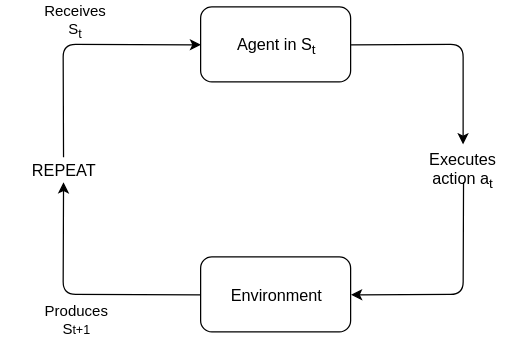
\includegraphics[scale=0.50]{Images/Reinforcement_Learning}
	\caption{\label{fig:Reinforcement Learning} The Reinforcement Learning Problem } 
\end{figure}

The definition of the state in a RL problem is very important for the success of the agent. The state should contain enough information so that the agent can fully utilize the information and make a decision. On the other hand it is unrealistic and unhelpful to define a state with more information than the agent should know at an expected point in time. This can be summarized to say that an agent is not expected to know everything important to it at all time points but is expected to remember anything that it has already experienced~\cite{sutton2018reinforcement}

Mathematically this is very similar to the Markov property which is commonly used in stochastic processes. Informally  the Markov property states that conditioned on the present value, the future value of the process is independent of the past values. For RL problems this means that the reward and the state signal that the agent will receive at time $t+1$ is only depends on the the state and action at time $t$. 

The Markov property is important as it allows one to calculate the dynamics of th transition to the next state purely based on the current state and action. A Markov system with a reward signal for transition from one state to another is known as a Markov Decision Process(MDP). The MDP tries to capture a world in the form of a grid by dividing it into states, actions, models, and rewards. The solution to an MDP is called a policy and the objective is to find the optimal policy for that MDP task. A RL task composed of a set of states, actions, and rewards that follows the Markov property would be considered an MDP~\cite{van2012reinforcement}. 

A \emph{finite} MDP is one in which the sets of states, actions and rewards all have finite number of elements. 
For a finite MDP the transition probabilities give the probability of transitioning from one state to another by taking some action. Let $s$ be the initial state, $a$ be the action and $s'$ be the subsequent state then the transition probabilities is given by.

\begin{equation}
	\mathbb{P}^a_{ss'} \ \dot{=} \  P(s_{t+1}=s' | s_t = s, a_t = a)
\end{equation}

And the expected reward of taking an action $a$ at time t depends only of the current state $s$ and the subsequent state $s'$.

\begin{equation}
\mathbb{R}^a_{ss'} = \mathbb{E} \big[r_{t+1} |s_{t+1} = s', s_t = s, a_t = a \big]
\end{equation}

The MDP framework is abstract and flexible and can be applied to different problems in different ways. Much of the current theory of RL is limited to the finite MDPs~\cite{sutton2018reinforcement}

\subsection{Elements of Reinforcement Learning Problem}

Beyond the agent, the environment and states there are other important elements of RL: a \emph{policy}, \emph{reward} signal, the \emph{value function}, and the \emph{action-value} function~\cite{sutton2018reinforcement}.


The policy defines the behaviour of the agent at any given time. It is the mapping of state, action pairs to the probabilities of selecting that action at each time step t. The aim of a RL algorithm is to specify how the agent should evaluate and update the policy given the experiences it has seen~\cite{sutton2018reinforcement}. The policy is usually represented by the symbol $\pi$


The reward signal defines the aim of the RL problem. The use of reward signal to define the idea of goal is one of the most distinctive features of RL. It might appear limiting at first to define the goal of the agent in terms of the reward signal, but in practice it has proved to be very flexible. At each time step the environment sends a single number to the RL agent called the reward. The reward signal defines the good and bad events for the agent ~\cite{sutton2018reinforcement}. The reward signal should be designed such that it accurately reflects the aim of the overall objective function rather than various sub-goals. An example of designing a simple reward function can be taken from an agent who is learning to play Chess. The reward can be +1 for a win, -1 for a loss and 0 for a tie. If we also assign reward signal for each of the opponents pieces captured, the agent will learn to focus on purely on capturing the opponents pieces rather than winning the aiming to win the game and therefore acting against its intended behaviour. 

As mentioned earlier the goal of the agent is to maximize the expected cumulative rewards. The expected cumulative rewards are called the \emph{expected returns}, where the return is defined as some function of the reward sequence. The simplest definition of return is the sum of the reward from a given time period to a terminal time period.

\begin{equation}\label{eq:reward}
G_t = R_{t+1} + R_{t+2} + R_{t+3} + \dots + R_{T}
\end{equation}

In ~\ref{eq:reward} T is the final time step. \ref{eq:reward} as defined guarantees that the agent will reach a terminal state, implying that T $< \infty$. These tasks are called \emph{episodic} tasks as they start in valid starting state, transitions through a finite of states and then reach a terminal state. However in many cases the agent-environment interaction can continue indefinitely i.e. T = $\infty$. These type of tasks are called \emph{continuing} tasks. \ref{eq:reward} cannot be used for continuing tasks as the sum can diverge to infinity and will be of little use to the agent. To counter this problem we use \emph{discounting}, which places more emphasis on immediate reward than it does to future rewards. We choose a parameter $\gamma \in [0,1]$ called the discounting parameter and the return is defined as.


\begin{equation}\label{eq:discounted_reward}
G_t  = R_t + \gamma^1 R_{t+1} + \gamma^2 R_{t+2} + \gamma^3 R_{t+3} + \dots = \sum_{k=0}^{\infty} \gamma^kR_{t+k+1}
\end{equation}\

The value of the discounting factor determines the present value of future rewards. If the value of $\gamma$ is zero then the agent is myopic i.e. it is concerned with maximizing only the current rewards. If the value of $\gamma$ the agent becomes more far-sighted and values immediate and future rewards equally. If $\gamma < 1$ then the infinite sum in \ref{eq:discounted_reward} has as finite value.



The \emph{value function} represents how good the state is for the agent to be in. It is equal to the expected total reward for an agent starting from the state \emph{s}. The value function is specific to the policy which the agent selects the action to perform. If the agent selects action from the policy $\pi$ in state \emph{s} then the value function is given by.

\begin{equation}\label{eq:value_function}
v_{\pi}(\emph{s}) = \mathop{\mathbb{E}}\bigg[\sum_{k=0}^{\infty} \gamma^k R_{t+k+1}\bigg | s_t = s]
\end{equation}

Among all the possible value functions there exists a an \emph{optimal value function} that has higher value than all the other value functions for all the states.

\begin{equation}\label{eq:optimal_value}
v^*_{\pi}(s) = max_{\pi} v_{\pi}(s) \hspace{1cm} \forall s \in \mathop{\mathbb{S}}
\end{equation}

In \ref{eq:optimal_value} $\mathop{\mathbb{S}}$ is the set of all possible states. The policy that corresponds to the optimal value function is called the optimal policy.

\begin{equation}\label{eq:optimal_policy}
	\pi^* = argmax_{\pi} v_{\pi}(s) \hspace{1cm} \forall s \in \mathop{\mathbb{S}}
\end{equation}

Solving a RL tasks roughly means finding a policy that achieves a lot of reward over the long run i.e. the optimal policy. 

Similar to the value function, the state action function defines the state action function or the \emph{Q function}. The Q function gives the expected return the agent will get starting from state $s$, taking action $a$ and thereafter following the policy $\pi$.

\begin{equation}
q_{\pi}(s,a) = \mathbb{E}_{\pi}\big[ G_t | S_t = s, A_t =a \big] = \mathbb{E}_{\pi}\big[\sum_{k=0}^{\infty} \gamma^k R_{t+k+1} | S_t = s, A_t = a\big]
\end{equation}

The value function $v_\pi$ and the action-value function $q_\pi$ are both estimated from experience. The fundamental problem that is used throughout RL to estimate the value and action-value function is that they satisfy recursive relationship~\cite{sutton2018reinforcement}. For any policy $\pi$ and any state s the following condition hold between the value of the state s and the value of the successor states.


\begin{equation} \label{eq:bellman}
\begin{split}
v_\pi &  \  \dot{=} \  \mathbb{E}_\pi \big[G_t | S_t = s\big] \\
& = \mathbb{E}_\pi \big[ R_t + \gamma G_{t+1} | S_t = s\big]\\
& = \sum_{a}^{} \pi(a|s) \sum_{s'}^{} \sum_{r}^{} p(s',r|s,a)\big[r + \gamma\mathbb{E}_\pi[G_{t+1} | S_{t+1} = s' ]\big] \\
& = \sum_{a}^{}\pi(a|s)\sum_{s',r} p(s',r|s,a)\big[r+ \gamma v_\pi(s') \big]
\end{split}
\end{equation}

\ref{eq:bellman} is the \emph{Bellman equation} for $v_\pi$ and it expresses the relationship between the value of a state and the value of its successor state. Bellman equation for the basis of a number of ways that can be used to compute $v_\pi$

\subsection{Solving Reinforcement Learning Problem}

The dynamics of the RL problem are not known and there are a large number of possible states therefore alternatives approaches are used to solve the reinforcement learning problem. Most methods use the Generalize Policy Iteration(GPI) to solve RL problems. 

GPI iteratively performs policy evaluation and policy improvement until sufficient convergence is observed. Policy Evaluation evaluates the value function for all the states with respect to the current policy. Policy improvement then uses these estimates to create a new policy that is greedy with respect to these estimates. The iteration are stopped when thee are no changes observed in the value function or the policy between iterations. It has been shown that the converged policy in GIP is actually the optimal policy. 

Different methods can be used for policy evaluation and improvement/ We will briefly discuss a few of them 

\begin{itemize}
	\item \textbf{Dynamic Programming(DP)} refer to a set of algorithms that can be used to compute the optimal policies given a perfect model of the environment as a MDP. DP algorithms recursively update the value function for each state by starting at that state and use the Bellman equation to update the values of all the states based on the expectation of their reward and the estimate of the values of the subsequent states. The process of using the estimates of values of the subsequent states to estimate the value of the current state is known as \emph{bootstrapping}. DP algorithms are of limited utility in RL both because of there assumptions of a perfect environment and because of their great computational cost~\cite{sutton2018reinforcement}.
	
	\item \textbf{Monte Carlo Methods} compute the optimal policy solely based on experience and do not require a full description of the environment, as long as we can produce sample runs from the environment. The value function is computed by averaging the return from each state over a number of sample runs also known as traces, until a convergence is reached. As we require each trace run to eventually terminate, Monte Carlo methods are only valid for episodic tasks. The policy is made greedy with respect to the value function computed and the algorithms repeats until it converges to the optimal policy.
	
	
	\item \textbf{Temporal Difference(TD) Learning} combine the best of DP and Monte Carlo methods. Like in DP they bootstrap by using the estimates to update other estimates. They also sample like Monte Carlo methods and do not require a full model of the environment to as they compute their estimates based on experienced runs. TD methods use the difference of value estimate for the states experienced at different points in time. TD methods do not wait until the end of an episode before updating their value estimates and thus can be used for non-episodic tasks.  
\end{itemize}

\section{Deep Reinforcement Learning}

